\section{Revising OpenStack}
\label{sec:leveraging-openstack}

OpenStack is an open-source project that aims at developing a complete cloud management
system. Similary to the reference architecture described in the previous Section, it is
composed of several services, each one dealing with a particular
aspect of a Cloud infrastructure as depicted in Figure~\ref{fig:openstack}.

\begin{figure}[htbp]
        \centering
        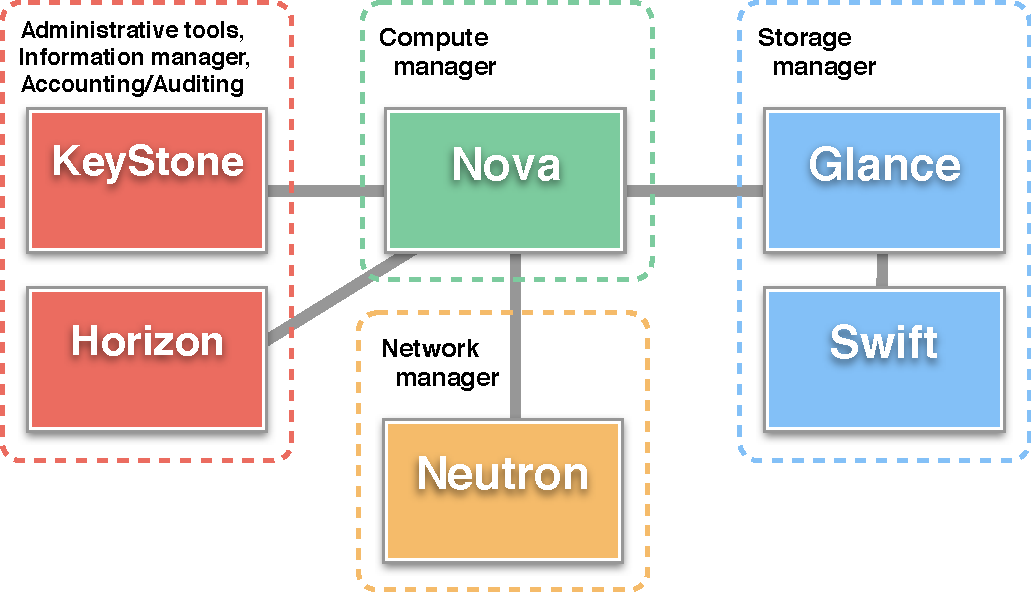
\includegraphics[width=6cm]{figures/OpenStack_architecture.pdf}
\vspace*{-.3cm}
        \caption{Services composing OpenStack.}
        \label{fig:openstack}
\vspace*{-.3cm}
\end{figure}


OpenStack relies on two kinds
of nodes: controller and compute node. The former is in charge of managing and
distributing work to the latter that provides computing/storage resources to end-users. In
other words, the controllers correspond to the different services introduced in the
previous section while the compute nodes host the VMs.

From the software point of view, the OpenStack architecture is based on the ``shared
nothing" principles: each controller (\ie each service) is connected to the others via two
different way:

\begin{itemize}
   \setlength{\itemsep}{0pt}
  \setlength{\parskip}{0pt}
   \setlength{\parsep}{0pt}
\item \textbf{A messaging queue} that enables the collaboration between sub-services of a
  controller.
\item \textbf{A SQL database} (DB) that stores inner states of a controller.
\end{itemize}

Finally, the controllers interact with each other through REST APIs or directly by accessing
the inner-state that are stored in the differents DBs.
%\AL[JP]{Is it correct ? How the controllers interaact/collabore ?}

Considering the current structure of OpenStack, the main limitation to make it distributed
is related to the SQL databases. Indeed, while OpenStack relies on the
RabbitMQ messaging service, which is articulated around a centralized
broker, there are few implementations of  P2P messaging
service such as ActiveMQ~\cite{activemq:2011} or ZeroMQ~\cite{zeromq:2013} that would be adapted to the LUC requirements.
% \section{Towards a fully distributed OpenStack deployment}
%
% The discovery initiative targets the delivery of an utility computing platform
% that will be working on top of existing network backbone facilities. Starting
% the development of such a platform from zero would require a titanic effort: in
% order to spare a giant development time, the Discovery initiative proposes to
% leverage the OpenStack project: this will serve as the foundation of the
% LUC-OS.
%
% In order to structure the LUC-OS on a fully distributed peer to peer
% functionning, OpenStack would be required to be fault tolerant and to be able to
% fit on a multi-site configuration. In the current situation, it requires some
% adaptations: in this section we propose some modifications that
% have been introduced in the Nova controller, to meet the two
% aforementioned criterions.
%
% \subsection{Replacing the relational backend by a Key/value store}
%
% From today's perspective, most of the OpenStack deployment are involving few
% nodes, thus not requiring more thant one controller. However, to meet the fault
% tolerance criterion, one needs to use \textit{High availibility} deployment by
% combining two components \textit{HAProxy} (load balancing) with
% \textit{Galera} (Relational database replication).
The first way to bypass the MySQL limitation is to
% a controller between distinct locations,
%\ie to be able to scale in/out the services it offers, is to
deploy each controller DB on each location and to synchronize the different DB
instances with a dedicated mechanism~\cite{kemme:vldb2010}. By such a mean, when a
controller processes a request and performs some actions on one site, changes in the
inner-state are also propagated to all the other locations. From a certain point of view,
it gives the illusion that there is only one DB for each service. Although the technique
described has been used in different proof-of-concepts, current DB synchronization
mechanisms are not scalable enough to cope with a LUC infrastructure deployed on large
number of geographical sites.

Another approach is to replace the DBs used in OpenStack by a more suitable storage
backend that would provide a better scalability. Distributed Hash Tables (DHTs) and more
recently key/value systems built on top of the DHT concept such as
\emph{Dynamo}~\cite{decandia:dynamo} have demonstrated their efficiency in terms of
scalability and fault tolerance properties.
%
In light of this, we have revisited the Nova controller, \ie the VM manager of OpenStack,
in order to to replace the current MySQL DB system by \textit{REDIS} ~\cite{han:2011},
a \textit{key/value store}.
% that extends the principles followed by the \textit{Dynamo}. %with more advanced storage and query features.
Technically speaking, we modified the Nova database driver. Indeed, the  Nova software architecture has been
organised in a way which ensures that each of its sub-services does not directly manipulate the database: they have an indirect
access through a service called ``nova-conductor" which in turn works with an
implementation of the \textbf{"nova.db.api"} programming interface. Developers of Nova
provide an implementation of this interface that is using \textit{SQLAlchemy} to
manipulate a relational database. We developed a second implementation of this interface
that replaces every call to the \textit{SQLAlchemy} by a call to a
custom key/value store
driver.  This enables  Nova's services to work with REDIS by only changing the
database driver, limiting the level of intrusiveness in the original source code.
Thanks to this modification, it is possible to instanciate  a distributed
cloud and operate it through a single instance of OpenStack composed
of several Nova controllers deployed on distinct sites.
Figure~\ref{fig:newnova} depictes such a deployment.
%
Each controller executes a REDIS instance that is configured to work in
a clustering way with other instances.
One or several controllers can be deployed on each site according to
the expected demand in terms of end-users. Finally, a controller can be
deployed either on a dedicated node or be mutalized with a compute
one as illustrated for Site 3. We higlight that any controller can
provision VMs by orchestrating services on the whole infrastructure and not only on the site
where it is deployed. Such a behavior is possible thanks to the AMQP
bus and the key/value store that go through all controllers.
%
Finally, it is noteworthy that key/value stores that
focus on high-availability and partition tolerance criteria like
Cassandra~\cite{lakshman:2010} would be more appropriate than REDIS
for a production deployment. We chose REDIS for its usage simplicity.

\begin{figure}[htbp]
        \centering
\vspace*{-.4cm}        \hspace*{-.2cm}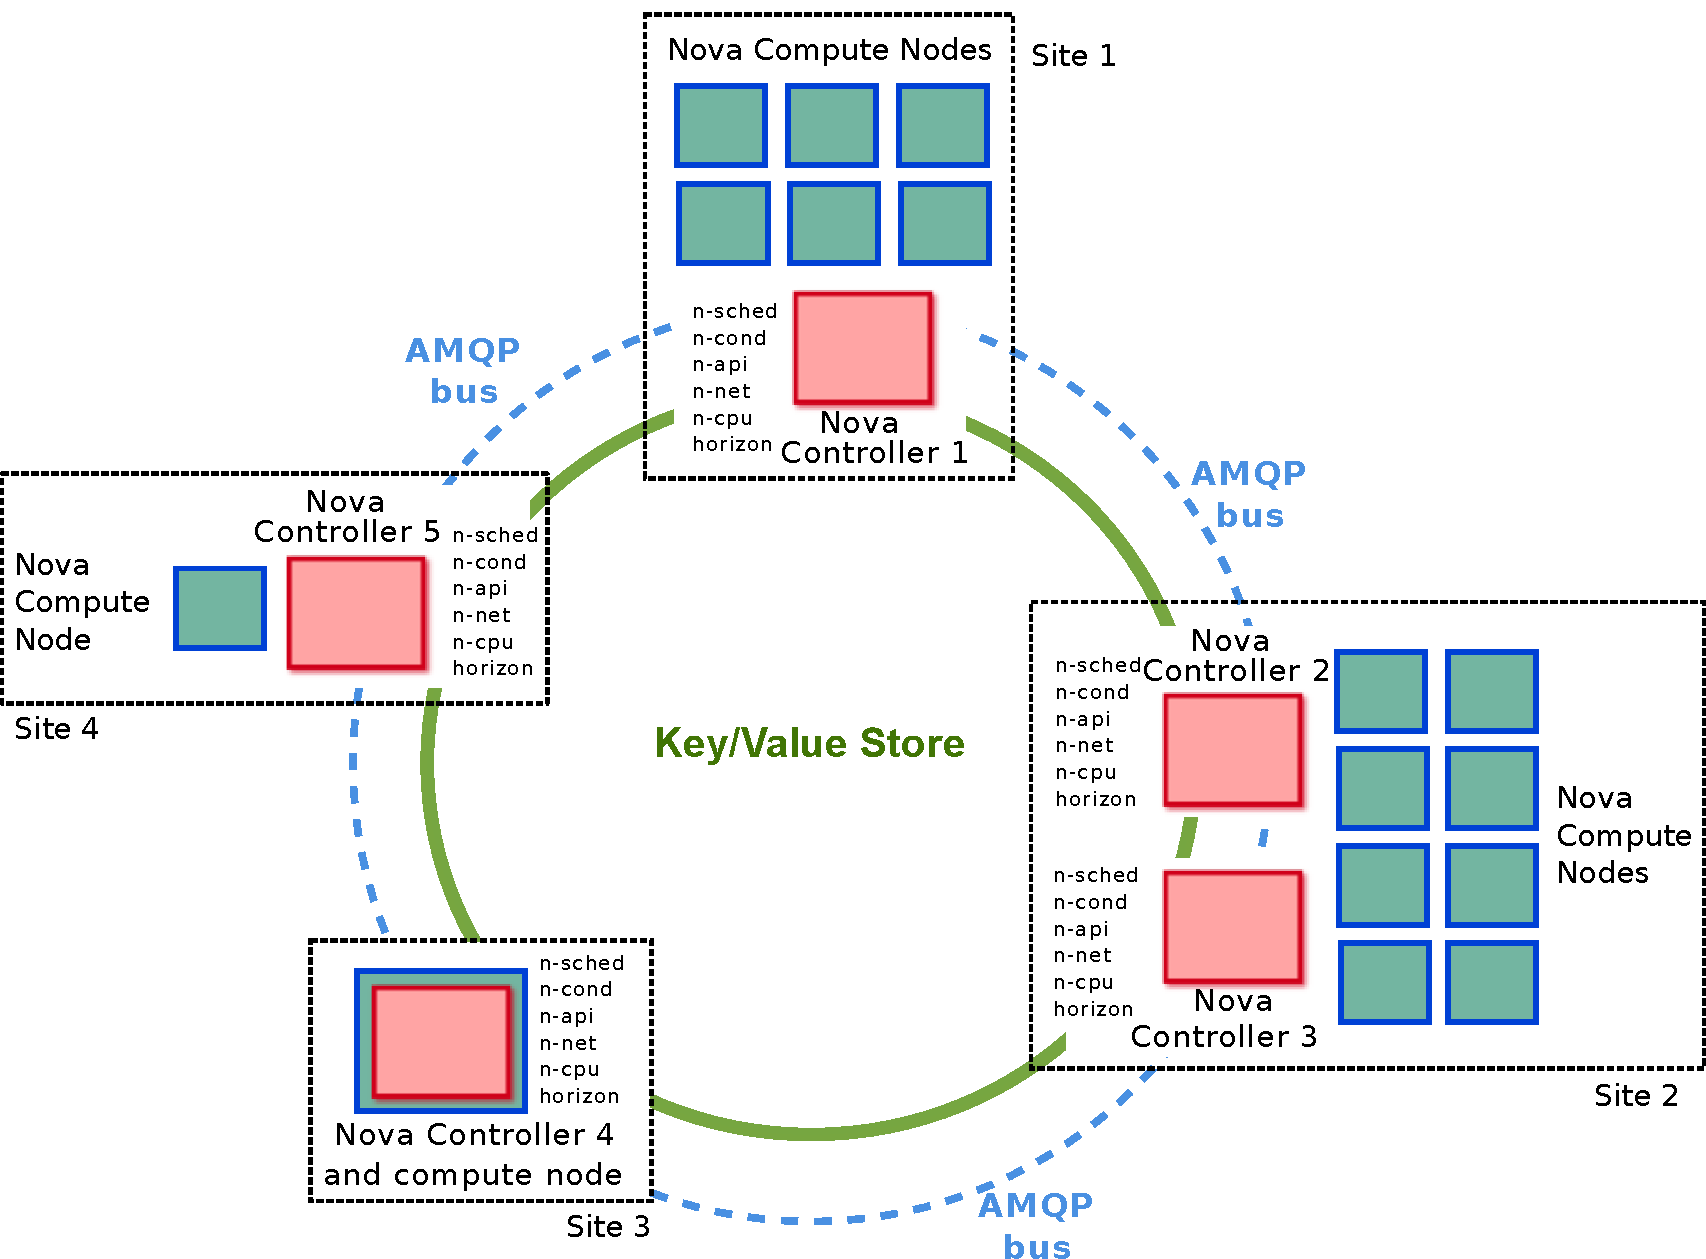
\includegraphics[width=.51\textwidth]{figures/OpenStack_distributed.pdf}
        \caption{Nova controllers are connected through a shared key/value backend
        and the AMQP bus.}
      \label{fig:newnova}
\vspace*{-.3cm}
\end{figure}

Our prototype is under evaluation.
However, preliminary experiments  have been performed throughout 4
sites of Grid'5000  including 12 compute nodes  and 4 controllers
overall. While this
infrastructure was rather small in comparison to our target, it aimed
at validating the interconnection of several controllers WANwide and
the correct behaviour of  OpenStack using our noSQL backend.
Our prototype suceeded to provision 500 VMs in 300 seconds
(each controller creating 125 VMs in parallel).
A second experiment validated the provisionning
of 2000 VMs in less than 30 min.  We are currently performing comparisons
between OpenStack using the historical MYSQL backend \textit{v.s.,}
using a key/value store backend. Our goal is to validate that
manipulating internal states of Openstack through
a noSQL deliver performances in the same order of the MySQL
ones.
